
\chapter{Unfolding}
\label{ch:unfolding}

This Chapter is a detailed treatment of \textit{unfolding}, a problem in particle physics data analysis that has been a primary focus of my Ph.D. research.
It will introduce the problem and why it is important in LHC physics, then illustrate conventional solutions that have been in use for many years.
Then it will turn to AI/ML based unfolding methods, highlighting a few methods that I played a role in developing.
These methods enable very high dimensional cross section measurements with many downstream physics applications.
The Chapter closes with an overview of the \Omnifold method.
This method is applied to experimental data to produce such a high dimensional cross section measurement in \Cref{ch:zjets}.

\section{Introduction to Unfolding}
\label{sec:unfolding-intro}

The detectors used in particle physics experiments are not perfect.
Every measurement they make has finite resolution and acceptance.
For example the ATLAS calorimeters are divided into calorimeter cells whose size place a firm lower bound on the angular resolution, and ATLAS as a whole has limited acceptance in the foward region because detectors cannot be placed inside the beampipe.
These imperfect measurements introduce \textit{detector effects} which must be accounted for in order to compare cross section measurements to theoretical predictions\footnote{Note that it is possible to neglect these effects if the measurement is performed in sufficiently coarse bins and in regions of phase space where acceptance effects are negligible. In this case the response matrix (see \Cref{sec:binned-unfolding-methods}) is completely diagonal and the detector-level and truth-level histograms are identical. These cases are rare because measurements are typically designed to make full use of the detector response, and so use finer binning and more inclusive phase space selection at the expense of introducing significant detector effects.}.
There are two general approaches to accounting for detector effects.
The first is \textit{forward folding} in which theoretical predictions, specifically a Monte Carlo (MC) event generator output that specifies the final state four-momenta of all long-lived particles produced in a collision, are passed through a simulation of the detector response and compared to the raw experimental data.
In this case the data and theoretical predictions are said to exist at \textit{detector level}, since the detector distortions are present in both.
The second strategy is \textit{unfolding}.
Instead of passing the theoretical preedictions through a detector simulation, statistical methods are used to construct an approximate inversion of the detector response, which is then applied to the data~\cite{Cowan:2002in}.
This removes detector effects from the measurement so that it can directly compared to theoretical predictions without passing the predictions through the detector simulation.
This process of removing distortions is called \textit{deconvolution} in other fields, since one can think of detector effects as the convolution of a noise function with the spectrum of interest
In the case that the unfolding adjusts only for detector distortions, the cross section measurement is said to exist at \textit{particle level}, since it makes a claim about the configuration of final state particles before interaction with the detector.
Some unfolding applications additionally account for the distortions produced by the parton shower and hadronization processes (see \Cref{ch:qcd}).
In this case the cross section measurement is said to exist at \textit{parton level}, since it makes a claim about the configuration of partons produced in the underlying hard scatter.
Both of these are unfolding and the methods discussed in this chapter apply to both.

In practice detector distortions are not the only effects that must be considered when unfolding.
A complete list is:
\begin{enumerate}[label={(\arabic*)}]
    \item Acceptance and efficiency: particles produced may not be measured.
    \item Detector noise: particles measured may not be from real particles, at least not the desired particles (e.g. fakes) within a fiducial volume (migrating into acceptance).
    \item Background processes: if one wants to measure the differential cross section of a particular process, then you may want to subtract the contributions from background processes.
    \item Combinatorics: if there are $n$ particles and you want to measure the properties of a particular order (e.g. leading $p_T$), the detector effects can change the order.
    \item Detector distortions: the detector response introduces bias and resolution effects.
\end{enumerate}
The unfolding in a well-structure measurement will primarily have to deal with (5).
For the measurement presented in \Cref{ch:zjets}, item (3) is dealt with but is a very sub-leading effect, and items (1,2,4) are irrelevant.
This is not generally the case for all particle physics measurements, but for the purposes of this thesis those items will be ignored as irrelevant effects.

Forward folding and unfolding are both actively used in cross section measurements an have distinct advantages and disadvantages.
Forward folding is strictly more precise than unfolding because unfolding methods will always incur additional systematic uncertainties.
These may be very sub-leading in which case the precision of both approaches is equivalent, but the unfolding approach will never be more accurate than forward folding\footnote{This claim is mostly true, but unfolded measurements can be more precise than forward folding if unfolding removes the need for some systematic uncertainties. This is sometimes the case for theoretical modeling uncertainties, where the difference between two MC generators is understood as an uncertainty for detector level spectra but only an arbitrary choice of prior for unfolded spectra. This ambiguity stems from the fact that modeling uncertainties are not true systematic uncertainties with a nuisance parameter that can be varied. Whether or not they should be included in a given context is often a somewhat philosophical question.}.
Despite this limitation, unfolding is often worth the added uncertainty for a few reasons which are worth spelling out in detail:

\begin{itemize}
    \item Unfolded measurements can be compared directly to theoretical predictions furnished by MC event generators without the need to pass the simulated events through the detector simulation. This is an enormous practical benefit. The general hope with any cross section measurement is that it will be used to improve our knowledge of particle physics, for example by constraining a free parameter of the Standard Model or tuning a hadronization model used to provide theoretical predictions. All of these downstream tasks are greatly simplified when detector simulation is not needed. For LHC datasets, the detector simulation is mostly proprietary, computationally expensive, and requires substantial expertise to run, making the forward folding approach inconvenient\footnote{Note that ``inconvenient'' can mean anything from hard to do within the personnel and funding constraints of a research group, to computationally infeasible with existing computational resources. Some downstream applications, for example fitting many Wilson coefficients of an effective field theory to measured spectra, require large amounts of simulation that may be impossible to produce at detector level.}. For legacy datasets, such as those produced by experiments at LEP or SLC, the detector simulation is no longer available, making the forward folding approach impossible. Unfolding can then be understood as a way of preserving cross section measurements for future unforeseen use cases, which might be understood only many years after the intial data taking of an experiment is complete.
    \item Unfolded measurements can be compared to non fully-inclusive theory predictions. In particular they can be compared to resummed calculations of jet substructure observables, which are defined at particle level but are represented as smooth functions rather than lists of final state particle four-momenta. This is an underappreciated motivation for unfolding. It is \textbf{required} to compare data to the rigourously understood theoretical predictions provided by state-of-the-art QCD calculations.
    \item Finally unfolded measurements are much easier to combine with other measurements, perhaps from different experiments, to exploit additional statistical power. Combining forward folded measurements is possible, but require access to the detector simulation for proper correlation of uncertainties. This becomes especially difficult if results from different experiments are combined. In contrast combining unfolded spectra is trivial. See Ref.~\cite{Heimel:2024drk} for an excellent example.
\end{itemize}

\begin{figure}[tb]
    \centering
    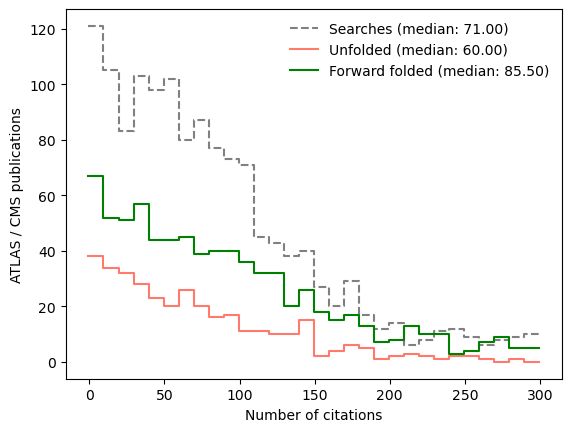
\includegraphics[width=0.66\linewidth]{figures/ch5/paper_citations.png}
    \caption{Histograms of all ATLAS and CMS physics results in the number of citations recieved. The tail of the distribution at very high citation counts is not shown. Histograms are shown for searches, measurements which forward fold, and measurements which unfold. Data scraped from the InspireHEP archive, and sorted based on keywords in abstracts and whether they cite key papers. Note these data are very approximate given unfolding is not always labeled explicitly.}
    \label{fig:paper-citations}
\end{figure}

Given these motivations may or may not apply depending on the goals of any measurement, the decision to use forward folding or unfolding is highly context specific.
It's worth mentioning a few contexts from LHC physics before moving on.
Searches for beyond-Standard-Model (BSM) particles almost never unfold.
Such searches look for coherent shapes like resonances in low-statistics regions of phase space, and unfolding would substantially reduce sensitivity.
It is true that a search using unfolded spectra would be vastly easier to re-interpret, but there is little practical motivation for doing this since well-established procedures exist within the experimental collaborations for re-interpreting searches via forward folding.
Among measurements of Standard Model processes, unfolding is used in roughly one third of published ATLAS and CMS measurements (excluding for example detector performance papers and searches), as illustrated in \Cref{fig:paper-citations}.
Extractions of parameters such as particle masses of Wilson coefficients typically do not unfold unless one of the goals of the result is to be used in combinations, while differential cross section measurements typically do.
This picture is complicated by the fact that some unfolded measurements are not described as such explicitly.
The Simplified Template Cross Section (STXS) framework used in ATLAS and CMS Higgs measurements~\cite{Berger:2019wnu}, for example, is an instance of profile likelihood unfolding (see \Cref{sec:binned-unfolding-methods}), but is rarely labeled as such in publications.
In summary, unfolding occupies a niche but important role in the LHC physics program, and is essential for data preservation and comparisons to resummed theory calculations.

\section{Binned Unfolding Methods}
\label{sec:binned-unfolding-methods}

Most cross section measurements report results as bin counts in histograms.
In this context, the unfolding task is to infer a truth-level histogram from the detector-level histogram produced by binning the data and a sample of simulated events for which both the truth-level and detector-level configurations are known.
These simulated events are used to construct a \textit{response matrix} that encodes how events migrate between bins at truth level and bins at detector level.

More formally, detector effects acting on a binned histogram can be modeled by the system of linear equations
\begin{align}
\label{eq:foldingequation}
\left(\textbf{R}\cdot (\textbf{t}\odot \textbf{c})\right)\odot 1/\textbf{f}+\textbf{b}=\textbf{d}\,,
\end{align}
where bold letters denote vectors or matrices, $\cdot$ is the usual matrix product, $\odot$ is the Hadamard (component-wise) product, and division is defined component-wise.\footnote{An equivalent way to write \Cref{eq:foldingequation} is $\left(\sum_{i}R_{ij}\,t_i\,c_i\right)/f_j+b_j=d_j$, where $i$ and $j$ are indices for the truth-level and detector-level bins, respectively.}
Here $\textbf{t}$ is the particle-level distribution, $\textbf{d}$ is the detector-level distribution, $\textbf{b}$ is the background contribution at detector level, and $\textbf{R}$ is the response matrix.
The correction factors $\textbf{c}$ account for events whose particle-level configuration passes the particle-level selection but whose detector-level configuration fails the detector-level selection (efficiency and acceptance losses corresponding to item (1) in \Cref{sec:unfolding-intro}).
The fake factors $\textbf{f}$ account for the inverse: events whose detector-level configuration passes the detector-level selection but whose particle-level configuration does not, corresponding to item (2).

The (maximum likelihood) solution to \Cref{eq:foldingequation} is
\begin{align}
\label{eq:unfolding}
\textbf{t}_\text{measured} = \textbf{R}^{-1}\left( (\textbf{d}-\textbf{b})\odot \textbf{f}\right)\odot 1/\textbf{c}.
\end{align}

In practice this direct matrix inversion is often not useful.
The response matrix $\textbf{R}$ is frequently ill-conditioned, meaning that its smallest singular values are close to zero.
Matrix inversion then amplifies statistical fluctuations in the detector-level histogram $\textbf{d}$ by a factor proportional to the condition number of $\textbf{R}$, producing a truth-level estimate with very large variance.
Put another way the naive algebraic solution to the unfolding problem can be highly numerically unstable.
Small changes in the detector level histogram (e.g. from statistical fluctuations) lead to large and unphysical oscillations in the unfolded histogram.
Most binned unfolding methods address this by deliberately injecting a small bias into the solution in order to reduce the variance, a procedure known as \textit{regularization} with conceptual ties to the bias-variance tradeoff discussed in \Cref{sec:ml-overview}.
In HEP applications this bias is typically estimated and propagated as a systematic uncertainty on the final result.
Reviews of binned unfolding methods in the context of high-energy physics can be found in Refs.~\cite{Cowan:2002in, Blobel:2011fih}.
A common feature of all methods is that they do not scale beyond unfolding a few simultaneous dimensions.
This is due to the curse of dimensionality, where the number of bins in a histogram grows exponentially with the number of dimensions making populating the bins of a high dimensional histogram intractable.
The inability of binned unfolding methods to scale to high dimensions is one motivation for unbinned unfolding, which will be discussed in the next Section.

\subsection{Profile Likelihood Unfolding}
\label{sec:plu}

Profile likelihood unfolding and its variants replace the naive matrix inversion solution with a likelihood model.
First write the expected detector-level bin counts as a function of the truth-level bin counts,
\begin{equation}
    \lambda_j = \sum_i^{N_t} R_{ij} t_i ,
    \label{eq:unfolding_expected_yield}
\end{equation}
with $R_{ij}$ the response matrix element for detector-level bin $j$ given truth-level bin $i$ and $N_t$ the number of truth-level bins.
Then assuming Poisson distributed bin counts, the log-likelihood is
\begin{equation}
    \mathcal{L}(\textbf{t} | \textbf{d}) = \log \prod_{j=1}^{N_d} \frac{e^{-\lambda_j}\lambda_j^{d_j}}{d_j!} = \sum_{j=1}^{N_d} \left( d_j \log \lambda_j - \lambda_j - \log d_j! \right) .
    \label{eq:unfolding_poisson_likelihood}
\end{equation}
where $N_d$ is the number of detector-level bins.
This replaces the linear system in \Cref{eq:unfolding} with a non-linear system that can be solved numerically.
Note that although there is no explicit inversion of the response matrix, if the response matrix is ill-conditioned then there are directions in $\textbf{t}$ where the likelihood is essentially flat at the same numerical issues can result.
This is why additional regularization of the likelihood is often required.
See for example Ref.~\cite{Tikhonov:1963}.

The principal advantage of this approach is that systematic uncertainties can be incorporated directly into the unfolding.
Each source of systematic uncertainty is represented by a nuisance parameter in the likelihood, which is then simultaneously constrained by the data together with the bin counts of the truth-level histogram.
This avoids the need to propagate systematic uncertainties by re-running the unfolding as is done in measurements performed with the IBU method in the next section.
The normalization of irreducible backgrounds can also be treated as a nuisance parameter and included in the unfolding.
The main drawback is that the regularization, though principled, can be delicate to tune in practice.
A common fix to these issues is to simply use coarser bins, so the response matrix is better conditioned but the measurement loses resolution.

Profile likelihood unfolding is becoming increasingly common in LHC analyses.
See for example Ref.~\cite{CMS:2024mke} or any Higgs boson measurements within the STXS framework, which is a prominent example of profile likelihood unfolding as noted in \Cref{sec:unfolding-intro}.
See Ref.~\cite{Collaboration:2944725} for an example of relatively high-dimensional profile likelihood unfolding with an explicit regularization term added to the likelihood.

\subsection{Iterative Bayesian Unfolding}
\label{sec:ibu}

Probably the most widely used binned unfolding method in HEP is \textit{Iterative Bayesian Unfolding} (IBU)~\cite{DAgostini:1994fjx}, also known as Lucy-Richardson deconvolution in other fields~\cite{Lucy:1974yx, Richardson:1972}.
IBU is an expectation-maximization (EM) algorithm, where a likelihood over the bin counts in both the dector-level and truth-level histograms is approximated with an expectation value (expectation step) and then maximized (maximization step).
Note the expectation step is required because we don't know the truth-level bin counts by construction.
Instead we have a prior furnished by MC simulation that is iteratively updated, which is why the method is referred to as Bayesian even though it is attempting to maximize a likelihood.
For clarity, the equations below assume $\textbf{b}=\textbf{0}$ and $\textbf{f}=\textbf{c}=\textbf{1}$, so that the folding equation reduces to $\textbf{R}\cdot\textbf{t} = \textbf{d}$.

Here the solution to one iteration of the expectation-maximization process will just be quoted without derivation.
The IBU estimate at iteration $n$ is
\begin{align}
t_i^{(n)}&=\sum_j \Pr(t_i|d_j)\, d_j \label{eq:ibu1}\\
&=\sum_j \frac{\Pr(d_j|t_i)\,\Pr^{(n)}(t_i)}{\sum_{i'} \Pr(d_j|t_{i'})\,\Pr^{(n)}(t_{i'})}\, d_j \label{eq:ibu2}\\
&=\sum_j \frac{R_{ji}\,\Pr^{(n)}(t_i)}{\sum_{i'} R_{ji'}\,\Pr^{(n)}(t_{i'})}\, d_j, \label{eq:ibu3}
\end{align}
where $\Pr^{(n)}(t_i) \propto t_i^{(n-1)}$ is the prior on the truth-level bin $i$ at iteration $n$, updated at each step using the estimate from the previous iteration.
The prior for the first iteration is taken from simulation, $\Pr^{(0)}(t_i) \propto t_i^{(0)}$.
It has been shown that as $n \to \infty$ the IBU estimate converges to the maximum likelihood estimator~\cite{Shepp:1982}.

The EM algorithm structure can be read off from these equations.
First, in \Cref{eq:ibu2} the current prior $\Pr^{(n)}(t_i)$ is held fixed and one calculates the posterior probability $\Pr(t_i | d_j)$ that a detector-level event in bin $j$ originated from truth-level bin $i$, using Bayes' theorem with the response matrix elements $R_{ji} = \Pr(d_j | t_i)$ as the likelihood.
This is the expectation step, since the method is calculating the expectation value of latent observables (how the events in bin $j$ of the detector-level histogram split across the truth-level bin $i$) given the current parameters $t_i^{(0)}$ and observations $d_j$.
The maximization step corresponds to the sum over $j$ and multiplication of the posterior probability by the detector-level bin counts $d_j$.
The posterior weights are used to redistribute the observed detector-level counts $d_j$ back to truth-level bins, yielding the updated estimate $t_i^{(n)}$, which then serves as the prior for the next iteration.
Because the number of iterations controls how far the estimate departs from the simulation prior, stopping the iteration early acts as the regularization mechanism in IBU.
Few iterations keep the result close to the prior corresponding to high regularization (high bias, low variance), while many iterations approach the maximum likelihood solution and zero regularization (low bias, high variance).

IBU is commonly used in HEP because it is flexible and easily interpretable.
Best practices for choosing when to stop the iterations have been documented and implemented in HEP specific software packages~\cite{Brenner:2019lmf}.
IBU is often the fastest and easiest way to get from detector-level to truth-level spectra.

\section{Unbinned and High-Dimensional Unfolding}
\label{sec:ai-unfolding-motivation}

The binned methods of \Cref{sec:binned-unfolding-methods} have been used in particle physics for decades but have limitations that bottleneck the flexibility of cross section measurements.
This section motivates adopting unbinned and high-dimensional unfolding techniques and surveys existing experimental applications.

\subsection{Motivation}
\label{sec:unbinned-motivation}

There are three key challenges of the binned unfolding methods, all of which can be addressed by unbinned and high-dimensional unfolding.
First, with binned methods the binning must be fixed before the analysis is complete and cannot be revised without introducing bias.
A binning optimized for one downstream application of the measurement will be suboptimal for another.
This is particularly relevant if one wishes to compute statistical moments of measured distributions, since binning introduces artifacts that will bias the result.
Unbinned unfolding avoids all of this by allowing the binning to be adjusted post-hoc or avoided entirely in the case of computing statistical moments.
This trick will be used extensively in \Cref{ch:zjets}.
Note that unbinned but low-dimensional unfolding methods have been proposed~\cite{Lindemann:1995ut, Aslan:2003vu, Glazov:2017vni}, as well as methods that target statistical moments directly~\cite{Desai:2024yft}.

The second challenge is dimensionality.
Conventional differential cross section measurements report a spectrum in a single observable, or at most two or three in a double or triple differential measurement.
As discussed in \Cref{sec:binned-unfolding-methods}, extending binned unfolding to more dimensions is impractical beyond three due to the curse of dimensionality.
High-dimensional unfolding removes this ceiling and allows for measurements of much more highly differential cross sections.
In practice this requires the unfolding be unbinned, and rely on machine learning methods since they are a natural tool for processing high-dimensional data.

The third challenge is that low-dimensional unfoldings do not take into account all possible auxiliary features that control the detector response.
This means that there can be ``hidden variables'' that the unfolding must marginalize over, which can limit the accuracy of the unfolding and increase unfolding uncertainties.
This is a subtle point, but the takeaway is that high-dimensional unfolding has the capacity to be more accurate than lower dimensional unfolding that can't take all available information into account.

A simple application of high-dimensional unfolding is to extend the length of the list of observables of interest to be anywhere from a handful to several tens.
This would produce a fixed but high dimensional cross section measurement that can be projected to any input observable to produce a measurement.
Additionally the correlations between observables would be preserved, so projecting to functions of the input observables is also supported.
Measurements of many observables can then be accomplished with a single analysis.
However the most ambitious application of high-dimensional unfolding is to extend the measurement to the full phase space, unfolding the kinematics of every particle measured by the detector.
This approach is maximally information preserving, in that the primary measurements actually made by the detector are corrected for detector effects rather than individual summary observables.
Note that because the number of particles produced in collisions is variable, this application defines a cross section measurement on a variable-dimensional space.
Such a measurement implicitly contains every observable computable from the final state, making the downstream application potential immense.
Future of observables of interest can be quickly measured and furture theoretical calculations can be quickly compared to data, without the need to conduct a new analysis, which can either be time and resource intensive or impossible if the detector simulation is no longer available.
Realizing this greatly increased flexibility and physics potential requires two major technical advances: machine learning methods powerful enough to unfold variable-length sets of particle four-momenta, and systematic uncertainties defined at the level of individual particle measurements.
The machine learning methods described below have already been shown to be capable of unfolding in high and variable dimensions.
The requirement for systematic uncertainties on individual particles is already satisfied for charged particles but difficult for neutral particles, which is why the measurement in \Cref{ch:zjets} uses charged particles only.
This also links directly to the bottom-up approach to systematic uncertainties in jet tagging discussed in \Cref{sec:constituent-top-tagging}.

\subsection{Experimental Results}
\label{sec:unbinned-experimental-results}

% Table: overview of experimental measurements using unbinned unfolding
% Based on Table I of arXiv:2507.09582 (Canelli et al.), with the addition of
% the ALEPH thrust measurement by the Electron-Positron Alliance (arXiv:2507.14349).
%
% Columns: Experiment | arXiv | Dimensions | Final State | Kinematic Selection
%
% NOTE: * denotes analyses where the reconstruction-level dimensionality spanned
%       the full phase space but the truth-level result is 8-dimensional.

\begin{table}
  \caption{%
    Overview of experimental measurements using unbinned unfolding methods,
    adapted from Ref.~\cite{Canelli:2025ybb} with the addition of the ALEPH thrust
    measurement~\cite{Electron-PositronAlliance:2025nbl}.
    For most results the unfolded dimensionality is the same at reconstruction
    and truth level; $*$ indicates analyses where the reconstruction-level
    dimensionality spanned the full phase space but the truth-level result is
    8-dimensional.
    Phase space definitions, including $\eta$ requirements, are given in
    the individual papers.
    Adapted under CC~BY~4.0.%
  }
  \label{tab:unbinned-unfolding-measurements}
  \centering
  \resizebox{\linewidth}{!}{%
  \begin{tabular}{@{} l l c l l @{}}
    \toprule
    Experiment & arXiv & Dim.\ & Final state & Kinematic selection \\
    \midrule
    ATLAS~\cite{ATLAS:2024xxl}
      & \href{https://arxiv.org/abs/2405.20041}{2405.20041}
      & 24
      & $Z$+jets
      & $p_{T}^{\ell\ell} > 200\,\text{GeV}$ \\
    ATLAS~\cite{ATLAS:2025qtv}
      & \href{https://arxiv.org/abs/2502.02062}{2502.02062}
      & 6
      & Dijets
      & $p_{T}^{j_{1}} > 240\,\text{GeV}$, $p_{T}^{j_{1}} < 1.5\,p_{T}^{j_{2}}$ \\
    CMS~\cite{CMS:2025sws}
      & \href{https://arxiv.org/abs/2505.17850}{2505.17850}
      & 8
      & Minimum bias
      & ${>}2$ charged particles, \pt $> 0.5\,\text{GeV}$ \\
    H1~\cite{H1:2021wkz}
      & \href{https://arxiv.org/abs/2108.12376}{2108.12376}
      & $8^{*}$
      & High-$Q^{2}$ DIS
      & $Q^{2} > 150\,\text{GeV}^{2}$ \\
    H1~\cite{H1:2023fzk}
      & \href{https://arxiv.org/abs/2303.13620}{2303.13620}
      & 10
      & High-$Q^{2}$ DIS
      & $Q^{2} > 150\,\text{GeV}^{2}$ \\
    H1~\cite{H1:2024mox}
      & \href{https://arxiv.org/abs/2412.14092}{2412.14092}
      & $8^{*}$
      & High-$Q^{2}$ DIS
      & $Q^{2} > 150\,\text{GeV}^{2}$ \\
    H1~\cite{H1:prelim}
      & --
      & var.
      & High-$Q^{2}$ DIS
      & $Q^{2} > 150\,\text{GeV}^{2}$ \\
    LHCb~\cite{LHCb:2022rky}
      & \href{https://arxiv.org/abs/2208.11691}{2208.11691}
      & 4
      & $Z$+hadrons in jets
      & $20 < p_{T}^{j} < 100\,\text{GeV}$, $p_{T}^{h} > 0.25\,\text{GeV}$ \\
    STAR~\cite{Song:2023sxb}
      & \href{https://arxiv.org/abs/2307.07718}{2307.07718}
      & 6
      & Jets
      & $20 < p_{T}^{j} < 50\,\text{GeV}$ \\
    STAR~\cite{Pani:2024mgy}
      & \href{https://arxiv.org/abs/2403.13921}{2403.13921}
      & 7
      & Jets (heavy ions)
      & $20 < p_{T}^{j} < 45\,\text{GeV}$ \\
    T2K~\cite{Huang:2025ziq}
      & \href{https://arxiv.org/abs/2504.06857}{2504.06857}
      & 6
      & Muon $+$ proton
      & $p_{p} > 450\,\text{MeV}$ (single transverse variables) \\
    \midrule
    ALEPH~\cite{Electron-PositronAlliance:2025nbl}
      & \href{https://arxiv.org/abs/2507.14349}{2507.14349}
      & 1
      & Hadronic $Z$ decays
      & $E_{ch} > 15$~GeV  \\
    \bottomrule
  \end{tabular}%
  }
\end{table}


A growing number of experimental measurements have now been performed using unbinned and high-dimensional unfolding methods.
\Cref{tab:unbinned-unfolding-measurements} summarizes these results.
All of them use the \Omnifold algorithm, which is described in detail in \Cref{sec:omnifold}.
The measurements span a range of collision systems, inlcuding $pp$, $ep$, $e^+e^-$, and neutrino scattering, illustrating that these methods are general purpose and not only for use in LHC experiments.
The ALEPH thrust measurement~\cite{Electron-PositronAlliance:2025nbl} is notable as a reanalysis of archival $e^+e^-$ data, demonstrating how unbinned unfolding enables new physics from legacy datasets.
The current record for the highest-dimensional cross section measurement is held by a preliminary H1 result~\cite{H1:prelim}, which targets the full final-state phase space of high-$Q^2$ DIS events with a variable-dimensional unfolding reaching a few hundred dimensions.
This is the first measurement of its kind and a proof of concept for the full phase-space program described above.
The remainder of the measurements in \Cref{tab:unbinned-unfolding-measurements} target fixed sets of observables ranging from 4 to 24 dimensions.
Only a handful of LHC measurements appear in this table, and many of the results listed are recent publications from 2024 and 2025.
Given the clear scientific motivation and the rapid maturation of the underlying methods, it is reasonable to expect this landscape to change substantially in the near future.

\section{Review of Existing Methods}
\label{sec:unfolding-methods}

For unbinned methods it is useful to recast the unfolding problem in continuous notation.
The forward folding equation of \Cref{eq:foldingequation} becomes
\begin{align}
\label{eq:folding-continuous}
p_{\mathrm{data}}(x) = \int p(x \mid z)\, p_{\mathrm{unfold}}(z)\, dz,
\end{align}
where $x$ denotes the detector-level event representation, $z$ the truth-level event representation, $p(x \mid z)$ the detector response (the conditional probability of observing $x$ at detector level given the truth-level configuration $z$), and $p_{\mathrm{data}}(x)$ the observed data distribution.
The goal of unfolding is to find the truth-level distribution $p_{\mathrm{unfold}}(z)$ such that smearing it through the detector response reproduces the data.
This is generally and ill-posed problem.
In the binned case this was visible in the ill-conditioned response matrix.
In the unbinned case the response function $p(x \mid z)$ is ``information destroying'', meaning that there are many different truth-level configurations that can produce the same detector-level configuration.

The EM iterations of IBU solve this equation in the discrete (binned) case.
The continuous analogs of \Cref{eq:ibu2,eq:ibu3} are
\begin{align}
\label{eq:ibu-continuous-estep}
p^{(n)}(z \mid x) = \frac{p(x \mid z)\, p^{(n)}(z)}{\int p(x \mid z')\, p^{(n)}(z')\, dz'}, \quad \text{(E-step)}
\end{align}
\begin{align}
\label{eq:ibu-continuous-mstep}
p^{(n+1)}(z) = \int p^{(n)}(z \mid x)\, p_{\mathrm{data}}(x)\, dx. \quad \text{(M-step)}
\end{align}
The E-step computes the posterior $p^{(n)}(z \mid x)$ via Bayes' theorem, using the current prior $p^{(n)}(z)$ and the detector response $p(x \mid z)$.
The M-step updates the truth-level distribution by marginalizing over $x$ under the observed data, weighted by the posterior just computed.
As in the binned case, the prior is initialized from simulation and updated at each iteration, and early stopping provides regularization.

All of the ML-based unfolding methods discussed in this section either directly solve the integral equation in \Cref{eq:folding-continuous} or use the EM procedure.
The first class of methods are in some sense unbinned generalizations of profile likelihood unfolding, and the second class are unbinned generalizations of IBU.
This is true in a precise sense for \Omnifold as will be shown in \Cref{sec:omnifold}.
This Section should illustrate that there are many unbinned and high dimensional unfolding methods available, all of which work~\cite{Huetsch:2024quz}.
What is needed is much more application to experimental data.

\subsection{Direct Methods}
\label{sec:direct-unfolding-methods}

\Cref{eq:folding-continuous} can be solved directly either with generative models that directly learn the relevant distributions or with likelihood ratio estimation via classifiers.
The generative approaches directly model the unfolded distribution as $q_\phi(z)$ and optimize $\phi$ so that samples from $q_\phi(z)$ match the data.
This requires a differentiable surrogate for the detector response $p(x \mid z)$, typically another generative model trained to approximate $q_\theta(x \mid z)$.
Since neural networks are differentiable by construction, gradients can flow through $q_\theta(x \mid z)$ allowing for the direct optimization of $q_\phi(z)$ using a log-likelihood loss as in \Cref{sec:generative}.
The models $q_\theta$ and $q_\phi$ can be optimized independently in sequence or jointly end-to-end~\cite{Vandegar:2020yvw, Butter:2025via}.
These methods are attractive for their direct approach and the ability to include nuisance parameters in the unfolding problem as with profile likelihood unfolding.
However the optimization can be difficult, especially in high and variable dimensional settings where point-cloud generative models must be trained.

The classifier based approach, which has only been recently explored, replaces the generative models with classifiers.
Dividing both sides of \Cref{eq:folding-continuous} by a reference density provided by MC simulation $p_{\mathrm{sim}}(x)$ yields a ratio equation that can be targeted with classifiers via the likelihood ratio trick discussed in \Cref{ch:ml}.
A novel loss function enforces that the estimated ratios satisfy the integral equation, providing a purely classifier-based route to solving the unfolding problem without EM iteration~\cite{Ore:2026qgp}.
This new method carries substantial promise because it only requires training classifiers but avoids the iterations of \Omnifold which can be very computationally expensive in practice.

\subsection{Generative Unfolding Methods}
\label{sec:generative-unfolding-methods}

A large class of ML unfolding methods performs EM, as in IBU, but replaces the binned response matrix with a learned generative model of the posterior $p(z \mid x)$ in the E-step.
Specifically these methods train a conditional generative model $q_\psi(z \mid x)$ to approximate the posterior in the left hand side of \Cref{eq:ibu-continuous-estep}.
A range of generative architectures have been studied for this purpose.
Early work used conditional variational autoencoders and generative adversarial networks~\cite{Datta:2018mwd, Howard:2021pos, Bellagente:2019uyp, Bellagente:2020piv}.
More recent work has moved to normalizing flows~\cite{Diefenbacher:2023wec, Butter:2024vbx} and diffusion and flow matching models~\cite{Butter:2025mek}, which offer improved expressiveness and the ability to scale to higher dimensional problems.
The choice of generative model for the posterior is the difference between all of these methods.
The underlying EM structure is common to all of them.
The diffusion and flow matching based methods I have contributed to are discussed in \Cref{sec:diffusion-unfolding}.

For the M-step, two implementations have been proposed.
The first reweights an MC simulation sample to match the posterior samples by training a classifier~\cite{Backes:2022sph}.
This is very similar to the second step of \Omnifold discussed below.
The second trains another generative model for the updated truth-level distribution $p^{(n+1)}(z)$ using the samples drawn from the posterior.
This approach requires passing samples from the updated truth-level distribution through the detector simulation, possibly via a surrogate model~\cite{Butter:2025mek}.

These methods are quite mature, but as of this writing none have been applied to experimental data.
This is partially because they require additional machine learning complexity (the training of generative models) but reduce to the same statistical procedure as the classifier based \Omnifold.
These methods do have lighter assumptions than \Omnifold on the support of the MC simulations used in the training, but it is unclear whether these assumptions are ever actually limiting for \Omnifold and how much better the generative model based approaches would perform if such a case were found.
This is doubly true because the same MC simulation support assumptions enter if the classifier based approach is used in the M-step.
The purely generative model based approach of Ref.~\cite{Butter:2025mek} is explicitly free of them, but still implicitly carries assumptions given generative models have difficulty generalizing out of distribution.
For another alternative, see Ref.~\cite{Acosta:2025shf} which forgoes the EM procedure entirely, and treats unfolding as a Bayesian problem with a fixed prior.
Despite these issues applications of methods that replace parts of the EM procedure with generative models should be pursued, since the pros and cons of different methods often only appear in realistic circumstances.

\subsection{Classifier-Based EM: OmniFold}
\label{sec:omnifold-preview}

The remaining class of methods performs EM but replaces the generative model for the posterior with likelihood ratio estimation via classifiers.
This is the approach taken by \Omnifold~\cite{Andreassen:2019cjw} and its variants~\cite{Chan:2023tbf, Zhu:2024drd}.
Given its central role in the experimental measurements reviewed in \Cref{sec:unbinned-experimental-results} and in the $Z$+jets measurement of \Cref{ch:zjets}, a full discussion of \Omnifold is reserved for that dedicated section.

\section{Unfolding with Diffusion and Flow Matching}
\label{sec:diffusion-unfolding}

\subsection{Variational Latent Diffusion Models}
\label{sec:vld-unfolding}

Ref.~\cite{Shmakov:2023kjj} was the first work to apply diffusion models to the generative unfolding task described in \Cref{sec:generative-unfolding-methods}.
It builds on the conditional invertible neural network (CINN) approach of Ref.~\cite{Bellagente:2020piv}, which used a normalizing flow as the generative model for the posterior $p(z \mid x)$ in the E-step of the EM procedure.
The normalizing flow is replaced with a \textit{variational latent diffusion} (VLD) model that performs the diffusion process in the latent space of a variational autoencoder (VAE), rather than directly in the high-dimensional event configuration space.

Latent diffusion models (LDMs) are roughly speaking the current state of the art in image generation tasks.
Ref.~\cite{rombach2022high} demonstrated that performing the diffusion process in the learned latent space of a pre-trained VAE, rather than directly in pixel space, reduces computational cost while maintaining or improving sample quality.
LDMs can also condition generation on inputs of different modality than the generated information.
For example contrastive learning objectives such as CLIP~\cite{radford2021learning} can align image and text embeddings, enabling the generation of images based on text inputs.
While such objectives were not employed in Ref.~\cite{Shmakov:2023kjj}, they were one reason we chose to use latent diffusion models since the detector-level event information plays a similar conditioning role for generations of the truth-level configuration.

However standard LDMs train the VAE and diffusion process independently.
The VAE is first trained to learn a latent representation of the data, then the weights of the VAE encoder and decoder are frozen and the diffusion model is subsequently trained within that fixed latent space.
This sequential approach limits the generative capacity of the combined model, since the VAE latent space is optimized solely for reconstruction rather than for the denoising objective.
Optimizing both jointly in a single end-to-end objective can in principle yield a latent representation that is better suited for the diffusion process.
Training both models simultaneously requires constructing a single ELBO that encompasses both the VAE and the diffusion model.

\subsubsection{The VLD Loss Function}

The VLD model is illustrated schematically in \Cref{fig:vld-diagram}.
Following the notation of \Cref{sec:generative-unfolding-methods}, let $x$ denote the truth-level event configuration and $y$ the detector-level event configuration.
The model introduces a latent variable $z_t$ parametrized by a continuous diffusion time $t \in [0, 1]$.
At $t = 0$, a sample $z_0$ is drawn from the VAE encoder posterior $q(z_0 \mid x, y)$.
The forward diffusion process then progressively corrupts $z_0$ with Gaussian noise so that $z_1$ is approximately distributed as the standard normal $p(z_1) = \mathcal{N}(0, I)$.
Given a trained model, samples from the posterior $p(x \mid y)$ are generated by running the learned reverse diffusion process conditioned on $y$, starting from a noise sample $z_1 \sim \mathcal{N}(0, I)$, and decoding the resulting $z_0$ back to parton-level quantities via the VAE decoder $p(x \mid z_0, y)$.

The VLD training objective combines this three-stage generative process (standard normal prior, diffusion, and VAE decoder) into one unified loss.
This is derived in the appendix of Ref.~\cite{Shmakov:2023kjj} and quoted here:
\begin{align}
    \mathcal{L}_{\text{VLD}}
    &= D_\text{KL}\!\left(q(z_1 \mid x, y) \;\|\; p(z_1)\right)
     + \mathbb{E}_{q(z_0 \mid x, y)}\!\left[-\log p(x \mid z_0, y)\right] \notag \\
    &\quad + D_\text{KL}\!\left(q(z_0 \mid x, y) \;\|\; p(z_0 \mid z_1)\right)
     + \mathbb{E}_{\substack{\varepsilon \sim \mathcal{N}(0, I) \\ t \sim \mathcal{U}(0,1)}}
       \!\left[\gamma_\phi'(t)\, \norm{\varepsilon - \hat{\varepsilon}_\theta(z_t, t, y)}^2\right].
    \label{eq:loss_lvd}
\end{align}
The first term is the prior loss, enforcing that the terminal diffusion state $z_1$ is close to the standard normal, analogous to the KL penalty in a standard VAE objective.
The second term is the VAE reconstruction loss, training the decoder to accurately recover $x$ from the latent $z_0$.
The third term is the novel contribution of the VLD framework: a KL divergence that regularizes the VAE encoder posterior $q(z_0 \mid x, y)$ against the first step of the reverse diffusion, $p(z_0 \mid z_1)$.
This additional term couples the VAE and the diffusion together, enabling the joint end-to-end optimization that distinguishes VLD from standard LDMs.
The fourth term is the diffusion denoising loss.
Translating to the notation of \Cref{sec:ddpm}, $\hat{\varepsilon}_\theta$ is the noise prediction network that predicts the noise $\varepsilon$ added to a latent sample $z_0$ at diffusion time $t$, and $\gamma_\phi'(t)$ is the derivative of the noise schedule.

\begin{figure}[t]
    \centering
    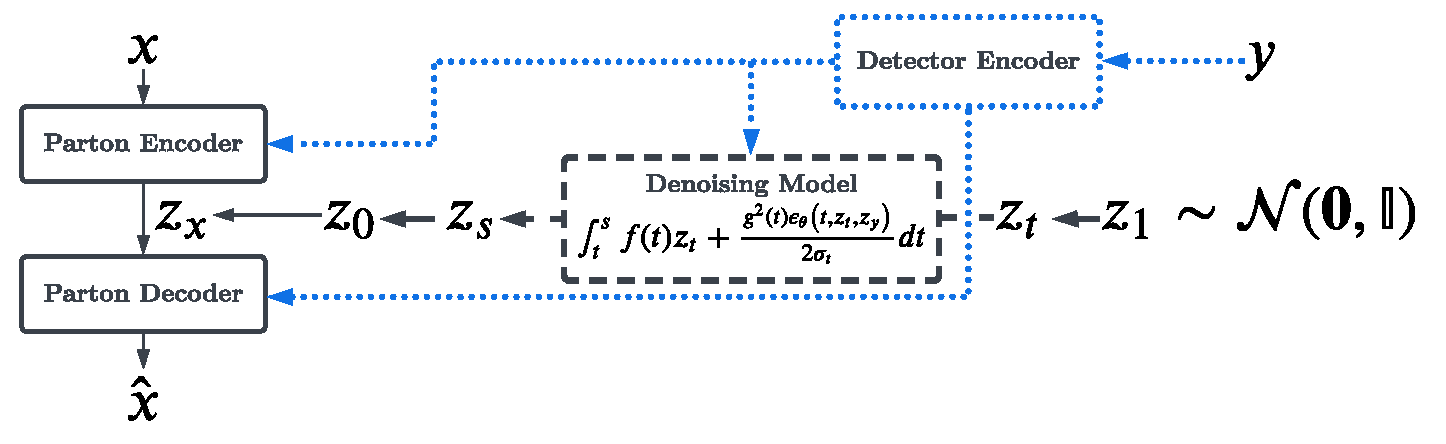
\includegraphics[width=0.88\linewidth, alt={Block diagram of the variational latent diffusion model showing the conditional detector encoder, parton VAE encoder, diffusion denoising network, and parton VAE decoder connected in a unified end-to-end architecture conditioned on detector-level information}]{figures/ch5/vld_diagram}
    \caption{Block diagram of the variational latent diffusion (VLD) model. The detector encoder (top right) embeds the detector-level event $y$ into a fixed-size latent vector that conditions the rest of the network. During training, the parton VAE encoder maps the truth-level event $x$ to a latent sample $z_0$, which the forward diffusion process noises to $z_t$. The denoising network predicts the added noise conditioned on $z_t$, the current time $t$, and the detector embedding. During inference the reverse diffusion process generates $z_0$ from $z_1 \sim \mathcal{N}(0, I)$, which the VAE decoder maps back to parton-level quantities. Figure reproduced from Ref.~\cite{Shmakov:2023kjj}.}
    \label{fig:vld-diagram}
\end{figure}

\paragraph{Noise schedule.}
Following Ref.~\cite{kingma2021variational} the noise schedule is learned through the parametrization
\begin{equation}
    \sigma_t^2 = \textrm(sigmoid)(\gamma_\eta(x))
    \label{eq:noise-schedule}
\end{equation}
where $\gamma_n(t)$ is a monotonic neural network with learned parameters $\eta$.
The variance-preserving diffusion process is used, so the schedule parameters map to the DDPM notation of \Cref{sec:ddpm} via
\begin{equation}
    \alpha_t^2 = 1 - \sigma_t^2
    \qquad \beta_t = 1 - \alpha_t .
    \label{eq:vld-schedule}
\end{equation}
The schedule is optimized jointly with the rest of the model throughout training, specifically to minimize the variance of the diffusion loss, the last term in \Cref{eq:loss_lvd}.
See the Appendix of Ref.~\cite{kingma2021variational} for more details.
At large $t$, $\gamma_\phi(t)$ is constrained to be large so that $\beta_t \approx 1$ and $z_1 \approx \mathcal{N}(0, I)$.
The derivative $\gamma_\phi'(t)$ appearing in the final term of \Cref{eq:loss_lvd} provides a weighting of the diffusion loss term that up-weights the contributions to the loss when the noise is changing rapidly.

\paragraph{Physics-informed consistency loss.}
An important practical challenge for generative unfolding in $t\bar{t}$ events is reproducing the sharply peaked invariant mass distributions of the hadronic $W$ boson, leptonic $W$ boson, hadronic top, leptonic top, and the full $t\bar{t}$ system, all of which correspond to known particle masses.
Generative models are known to struggle with such narrow distributions.
To address this, a physics-informed consistency loss is added to the reconstruction objective.
It penalizes deviations from the relativistic energy-momentum relation $E^2 = \norm{\mathbf{p}}^2 + M^2$ for each predicted particle.
Defining $\hat{E}$, $\hat{\mathbf{p}}$, and $\hat{M}$ as the network's predicted energy, momentum, and mass of a given particle, the consistency loss is
\begin{equation}
    \mathcal{L}_C = \lambda_C\,\abs{\hat{M}^2 - \bigl(\hat{E}^2 - \norm{\hat{\mathbf{p}}}^2\bigr)},
    \label{eq:vld-consistency}
\end{equation}
with hyperparameter $\lambda_C$ controlling the relative weight.
The total reconstruction loss is the sum of the MSE reconstruction loss and $\mathcal{L}_C$.
This constraint was found to be essential for reproducing sharp mass peaks.

\subsubsection{Model Architecture}

The architecture of each component is kept deliberately simple.
The detector encoder follows the gated transformer design of SPANet~\cite{Shmakov:2021qdz}, given the detector-level condition should be permutation invariant.
The remaining components — the parton VAE encoder, the parton VAE decoder, and the denoising network — are all feedforward networks built from a gated inverted-bottleneck block structure.
More advanced set-processing architectures for the parton-level components are not necessary because the method is restricted to fixed-dimensional unfolding tasks where the parton-level configuration is a fixed-length vector.

\subsubsection{Unfolding Semi-leptonic $t\bar{t}$ Events}

The VLD model is evaluated on parton-level unfolding of semi-leptonic top quark pair ($t\bar{t}$) production.
Top quarks are frequently produced in pairs at the LHC and each decays to a $W$ boson and a $b$ quark.
In the semi-leptonic channel, shown in \Cref{fig:ttbar-feynman}, one $W$ decays hadronically to two light quarks and the other decays leptonically to a charged lepton and a neutrino.
The parton-level unfolding target consists of the four-momenta of the six final-state partons together with the four-momenta of the four intermediate resonances ($W_\text{had}$, $W_\text{lep}$, $t$, $\bar{t}$) and the $t\bar{t}$ system.
Each of the 11 particles is represented by five quantities $(M, \log E, p_x, p_y, p_z)$, giving a 55-dimensional parton-level space.

\begin{figure}[t]
    \centering
    \tikzset{
        photon/.style={decorate, decoration={snake}, draw=red},
        electron/.style={draw=blue, postaction={decorate},
            decoration={markings, mark=at position .55 with {\arrow[draw=blue]{>}}}},
        gluon/.style={decorate, draw=magenta,
            decoration={coil, amplitude=4pt, segment length=5pt}}
    }
    \begin{tikzpicture}[
        thick,
        % \ifarxiv 
        % scale=0.85,
        % \else
        scale=0.80,
        % \fi
        % Set the overall layout of the tree
        level/.style={level distance=1.2cm},
        level 2/.style={sibling distance=1.6cm},
        level 3/.style={sibling distance=1.2cm}
    ]
    \coordinate
        child[grow=left]{
            child {
                node {$g$}
                % The 'edge from parent' is actually not needed because it is
                % implicitly added.
                edge from parent [gluon]
            }
            child {
                node {$g$}
                edge from parent [gluon]
            }
            edge from parent [gluon] node [above=3pt] {$g$}
        }
        % I have to insert a dummy child to get the tree to grow
        % correctly to the right.
        child[grow=right, level distance=0pt] {
        child  {
            child {
                child {
                    node {$\bar{d}$}
                    edge from parent [electron]
                }
                child {
                    node {$u$}
                    edge from parent [electron]
                }
                edge from parent [photon] node [below=3pt] {$W$}
            }
            child {
                node {$b$}
                edge from parent [electron]
            }
            edge from parent [electron]
            node [below] {$t$}
        }
        child {
            child {
                node {$\bar{b}$}
                edge from parent [electron]
            }
            child {
                child {
                    node {$\bar{v}$}
                    edge from parent [electron]
                }
                child {
                    node {$e^{-}$}
                    edge from parent [electron]
                }
                edge from parent [photon] node [above=3pt] {$W$}
            }
            edge from parent [electron]
            node [above] {$\bar{t}$}
        }
    };
\end{tikzpicture}
    \caption{Feynman diagram for semi-leptonic $t\bar{t}$ production. Each top quark decays to a $W$ boson and a $b$ quark. Here the hadronic $W$ decays to $u\bar{d}$, and the leptonic $W$ decays to $e^- \bar{\nu}$. The unfolding target is the set of four-momenta of all six final-state partons ($b$, $\bar{b}$, two light quarks, the charged lepton, and the neutrino) along with the four intermediate resonances and the $t\bar{t}$ system.}
    \label{fig:ttbar-feynman}
\end{figure}

\paragraph{Dataset and training.}
Training and testing samples are generated with Monte Carlo simulation at $\sqrt{s} = 13$~TeV.
Matrix elements are evaluated using \textsc{MadGraph\_aMC@NLO}~\cite{Alwall:2014hca} with a top mass of $m_t = 173$~GeV.
Parton showering and hadronization are performed with \textsc{Pythia8}~\cite{Sjostrand:2014zea} and detector response is approximated using \textsc{Delphes}~\cite{deFavereau:2013fsa} with the CMS detector card.
Jets are clustered with the anti-$k_t$ algorithm~\cite{Cacciari:2008gp} with radius parameter $R = 0.5$.
Events are required to contain exactly one lepton and at least four jets with $p_T > 25$~GeV and $|\eta| < 2.5$, of which at least two must be $b$-tagged.
Approximately 9.9 million events are used for training and 1.3 million for testing.

\paragraph{Baseline models.}
The VLD variants are compared against five baselines.
The CVAE and CINN~\cite{Bellagente:2020piv} represent the prior state of the art in generative unfolding.
Two ablations isolate specific VLD components: the VDM operates the diffusion directly in the 55-dimensional parton space without any latent compression, and the LDM uses a pre-trained (independently optimized) VAE rather than the jointly trained one.
Additional ablations of the VLD conditional encoder and decoder (C-VLD and UC-VLD) test the effect of conditioning the VAE on the detector embedding.

\subsubsection{Results}

\Cref{tab:vld-distances} presents distribution-free distances between the models' unfolded samples and the truth-level distributions, summed across all 55 parton-level dimensions.
Three families of distance metrics are reported: the Wasserstein and energy distances (bin-independent measures based on the empirical cumulative distribution function), the Kolmogorov-Smirnov test statistic, and empirical KL divergences computed with 64, 128, and 256 bins.
The jointly trained VLD variants (VLD and UC-VLD) achieve the best performance by a wide margin across nearly all metrics, with total Wasserstein distances of 108.8 and 73.6 respectively, compared to 402 for the independently pretrained LDM.
All latent-space models substantially outperform the direct parton-space methods (CINN and VDM), showing the higher expressivity of latent diffusion.

\begin{table}[t]
    \caption{Total distribution-free distance metrics, summed across all 55 parton-level components, for each generative model. Lower values indicate better agreement with the truth distribution. Bold entries mark the best performance in each column. The VLD variants are the proposed jointly trained models; LDM is the pre-trained latent baseline; CINN~\cite{Bellagente:2020piv} is the normalizing-flow baseline; VDM and CVAE are non-latent baselines.}
    \label{tab:vld-distances}
    \centering
    \begin{tabular}{lrrrrrr}
\toprule
 & Wasserstein & Energy & K-S & $KL_{64}$ & $KL_{128}$ & $KL_{256}$ \\
\midrule
\textbf{VLD} & 108.76 & 7.59 & 4.08 & \textbf{3.47} & \textbf{3.74} & \textbf{4.53} \\
\textbf{UC-VLD} & \textbf{73.56} & \textbf{6.35} & \textbf{3.41} & 5.77 & 7.10 & 8.48 \\
\textbf{C-VLD} & 389.62 & 25.39 & 4.65 & 9.54 & 10.09 & 10.79 \\
LDM & 402.32 & 24.09 & 5.91 & 14.71 & 16.34 & 17.92 \\
VDM & 2478.35 & 181.35 & 17.14 & 29.28 & 32.29 & 35.60 \\
CVAE & 484.56 & 32.29 & 6.37 & 7.79 & 9.17 & 10.60 \\
CINN & 3009.08 & 185.13 & 15.74 & 28.55 & 30.19 & 32.37 \\
\bottomrule
\end{tabular}
\end{table}

\Cref{fig:particle-highlights} shows the global unfolded distributions for a selection of parton-level components.
The VLD model faithfully reproduces the truth distributions across a wide range of kinematic quantities, including the narrow invariant mass peaks of the top quarks and $W$ bosons.
The closure is not perfect, but a generative model based unfolding of parton-level mass peaks is very ambitious.
This performance was state of the art at the time.
The non-latent baseline CINN and the pre-trained LDM produce significantly worse mass peaks.
The CINN predictions are shifted and signficantly broader than the group truth, perhaps because of the invertibility requirement in flow based models.
The LDM model actually produces overly sharp mass peaks compared to truth.

\begin{figure}[t]
    \centering
    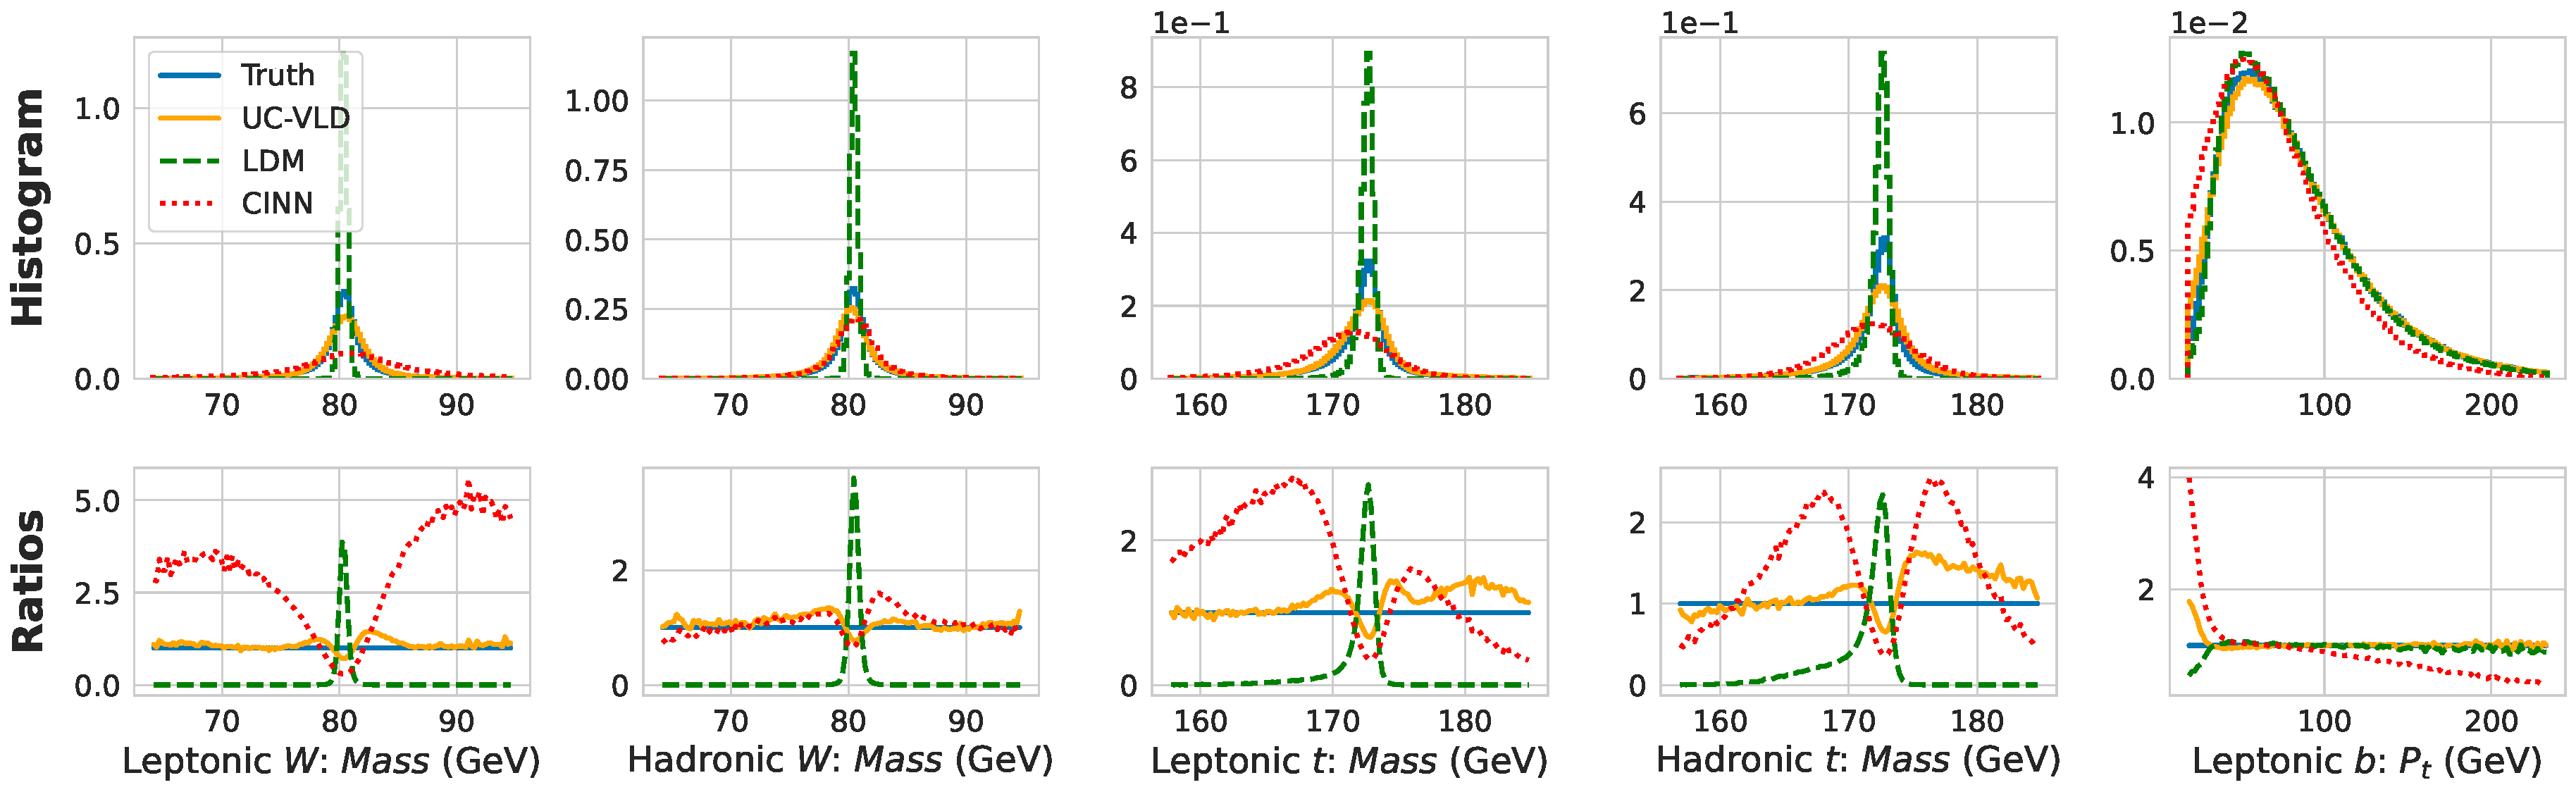
\includegraphics[width=\linewidth, alt={Comparison of unfolded kinematic distributions for selected parton-level components including top quark masses energies and W boson masses comparing VLD UC-VLD LDM CINN and VDM models against truth distributions with ratio panels}]{figures/ch5/particle_highlights}
    \caption{Highlighted unfolded distributions for selected parton-level components. Upper panels show the predicted and truth-level global distributions; lower panels show the ratio of predicted to truth. The VLD models accurately reproduce the sharply peaked invariant mass distributions of the top quarks and $W$ bosons, while baseline models exhibit smeared or shifted peaks. Figure from Ref.~\cite{Shmakov:2023kjj}.}
    \label{fig:particle-highlights}
\end{figure}

\subsubsection{Per-Event Posterior Distributions}

Though the learned posterior $q_\phi(z \mid x)$ is typically marginalized over $x$ as in \Cref{eq:ibu-continuous-mstep}, it is still interesting to examine the per-event posterior distributions produced by the model.
By drawing multiple samples from the trained model conditioned on a single detector-level event $y$, one can map out the full posterior $p(x \mid y)$ for that event.
This \textit{oversampling} can also be useful in the broader unfolding task, since it can amplify the statistics of small data samples~\cite{Butter:2020qhk}.
\Cref{fig:vld-posteriors} shows example per-event posteriors for several events and parton-level components.
The most striking feature is the bimodal posterior in the neutrino pseudorapidity $\eta_\nu$.
Neutrinos escape the detector without interacting, so their kinematics can only be inferred indirectly from the event's missing transverse momentum.
The neutrino's longitudinal momentum is further constrained by requiring the leptonic $W$ to satisfy its on-shell mass condition, which gives rise to a quadratic equation in the neutrino longitudinal momentum.
This equation generically admits two solutions, so two neutrino configurations are often simultaneously consistent with energy and momentum conservation for the same detector-level event.
The VLD model appears to have learned this ambiguity from the training data and produces a bimodal posterior that represents both physically valid solutions.

\begin{figure}[t]
    \centering
    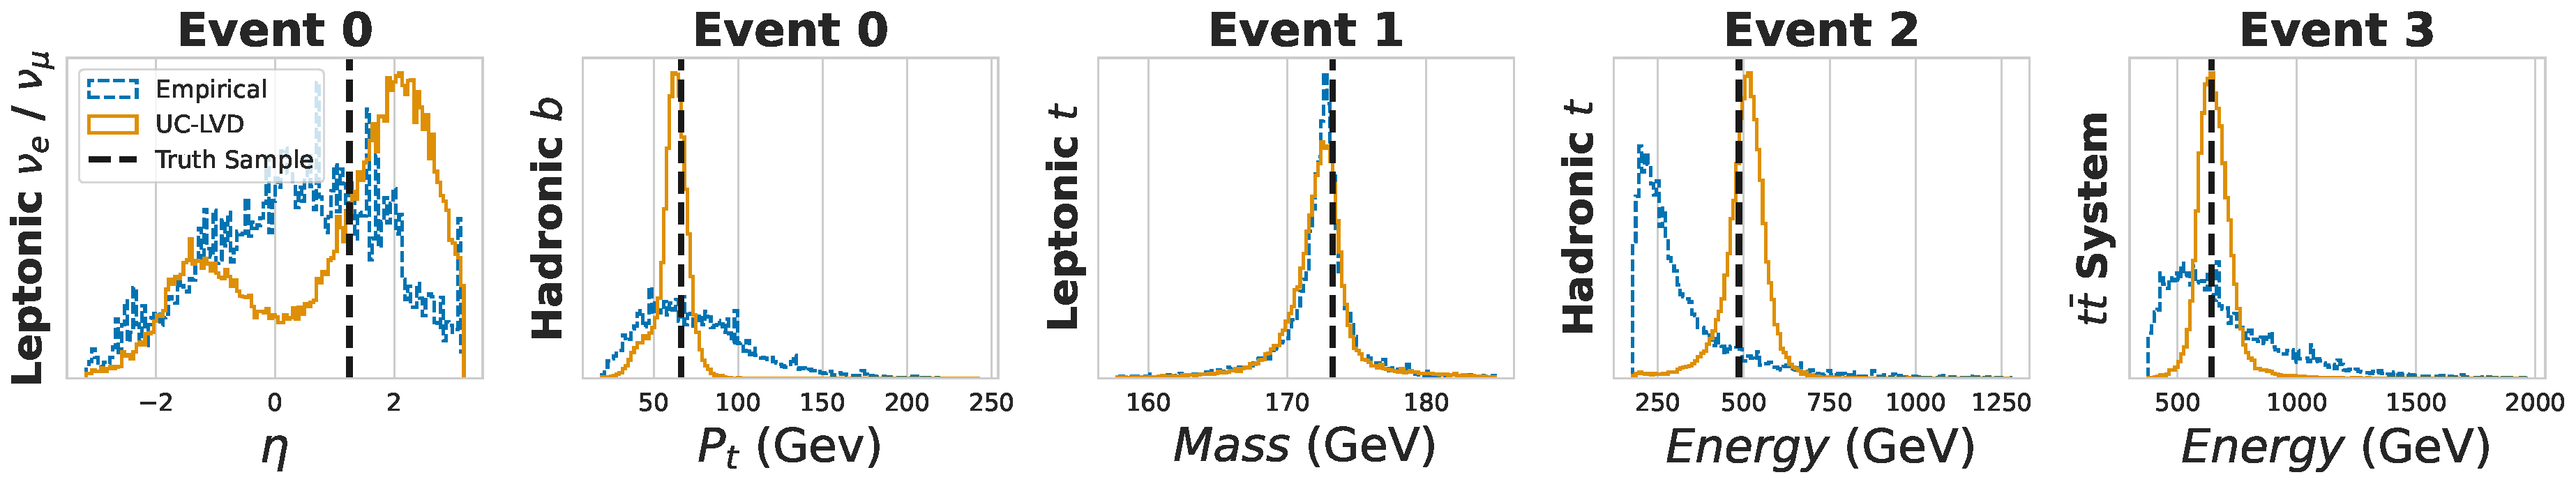
\includegraphics[width=\linewidth, alt={Per-event posterior distributions for selected parton-level components from several example events showing the VLD model posterior compared against an empirical brute-force estimate with the neutrino pseudorapidity showing a bimodal structure}]{figures/ch5/posterior_interesting}
    \caption{Highlighted per-event posterior distributions for several example events and parton-level components. The VLD model posteriors (orange) are compared against an empirical brute-force posterior estimate (blue) derived from the training data via exponential distance weighting. The neutrino pseudorapidity $\eta_\nu$ displays a clear bimodal structure in the VLD samples, reflecting the two solutions to the on-shell $W$ mass constraint on the neutrino longitudinal momentum. Figure from Ref.~\cite{Shmakov:2023kjj}.}
    \label{fig:vld-posteriors}
\end{figure}

\subsubsection{Summary and Key Contributions}

Ref.~\cite{Shmakov:2023kjj} makes three primary contributions to generative unfolding.
First, it is the first work to apply diffusion models to the problem of modeling the posterior in an unfolding task, establishing a new class of generative architectures for this problem.
Second, the unified end-to-end VLD training objective achieves state-of-the-art performance relative to all prior generative unfolding methods, with distribution-free distances over 20 times smaller than the non-latent state of the art and over three times smaller than a pre-trained latent diffusion baseline.
Third, by simultaneously unfolding all 55 dimensions of the $t\bar{t}$ parton-level space, the work represented the highest-dimensional generative unfolding demonstrated at the time of its publication.

\subsection{Variable Length VLD}
\label{sec:vl-vld}

\subsection{Unfolding Jet Substructure with Flow Matching}
\label{sec:cfm-jets}

\section{Omnifold}
\label{sec:omnifold}

